\documentclass[output=paper]{langsci/langscibook} 
\author{Andy Lücking\affiliation{Goethe-Universität Frankfurt}}
\title{Gesture}

% \chapterDOI{} %will be filled in at production

\epigram{% 
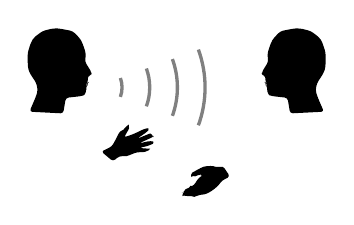
\begin{tikzpicture}[scale=1.1,
  iam/.style={draw=gray, thick, ellipse, font=\scriptsize,
    text=white, align=center, inner sep=2pt, fill=gray!60},
  conn/.style={draw=gray!80,thick},
  hypconn/.style={draw=gray!80, dashed, thick},
  trans/.style={draw=gray!80, very thick,
    shorten <=2pt, shorten >=2pt, dotted},
  % background rectangle/.style={fill=gray!30},
  % show background rectangle
  ]  
  % head:      
  \fill[color=black,rounded corners=1pt] (0.05,0.02) .. controls (0.15,0.25) .. (0.13,0.35) .. controls (0.03,0.5) .. (0.03,0.7) .. controls (0.08,0.86) .. (0.2,0.95) .. controls (0.35,0.99) .. (0.55,0.95) .. controls (0.65,0.85) .. (0.7,0.7) -- (0.7,0.65) -- (0.69,0.6) -- (0.77,0.47) -- (0.76,0.44) -- (0.72,0.43) -- (0.73,0.36) -- (0.71,0.35) -- (0.72,0.33) -- (0.7,0.3) -- (0.71,0.25) .. controls (0.68,0.21) .. (0.65,0.2) -- (0.47,0.18) -- (0.44,0) -- cycle;
  % Schallwellen:
  \draw[very thick,color=gray,decorate,decoration={expanding waves,angle=20}] (0.8,0.3) -- (2.1,0.3); 
  %%%%%%%%%%%%%%%%%%%%%%%%%%%%%%%%%%%%%%%%%%%%%%%%%%%%%%%%%%%% 
  % right interlocutor:
  \begin{scope}[xshift=3.5cm]
    \pgftransformxscale{-1}
    % network
    % head  
    \fill[color=black,rounded corners=1pt] (0.05,0.02) .. controls (0.15,0.25) .. (0.13,0.35) .. controls (0.03,0.5) .. (0.03,0.7) .. controls (0.08,0.86) .. (0.2,0.95) .. controls (0.35,0.99) .. (0.55,0.95) .. controls (0.65,0.85) .. (0.7,0.7) -- (0.7,0.65) -- (0.69,0.6) -- (0.77,0.47) -- (0.76,0.44) -- (0.72,0.43) -- (0.73,0.36) -- (0.71,0.35) -- (0.72,0.33) -- (0.7,0.3) -- (0.71,0.25) .. controls (0.68,0.21) .. (0.65,0.2) -- (0.47,0.18) -- (0.44,0) -- cycle;
    % Schallwellen:
    % \draw[very thick,color=gray,decorate,decoration={expanding waves,angle=25}] (0.8,0.3) -- (1.3,0.3); 
  \end{scope}
  %% Hand links
  \begin{scope}[scale=0.55,xshift=1.6cm,yshift=-0.8cm,rotate=320]
    \fill[color=black,rounded corners=1pt] (0,0) -- (0.1,0.22) .. controls (0.08,0.35) .. (0.05,0.46) .. controls (0.03,0.56) .. (0.05,0.63) .. controls (0.06,0.65) .. (0.06,0.75) .. controls (0.07,0.78) and (0.14,0.78) .. (0.15,0.65) .. controls (0.18,0.54) .. (0.3,0.75) .. controls (0.35,0.87) .. (0.4,0.97) .. controls (0.43,1) and (0.47,0.98) .. (0.47,0.93) -- (0.4,0.68) .. controls (0.54,0.95) .. (0.6,0.97) .. controls (0.61,0.96) and (0.64,0.96) .. (0.62,0.9) -- (0.49,0.63) .. controls (0.58,0.75) .. (0.65,0.84) .. controls (0.72,0.87) and (0.72,0.81) .. (0.7,0.77) .. controls (0.66,0.7) .. (0.56,0.57) .. controls (0.65,0.63) .. (0.7,0.67) .. controls (0.74,0.7) and (0.78,0.63) .. (0.58,0.47) .. controls (0.47,0.26) .. (0.35,0.17) .. controls (0.33,0.05) .. (0.32,0) -- cycle;
  \end{scope}
  %%%%%%%%%%%%%%%%%%%%%%%%%%%%%%%%%%%%%%%%%%%%%%%%%%%%%%%%%%%% 
  % Hand rechts
  \begin{scope}[scale=0.55,xshift=3.3cm, yshift=-1.75cm]
    \fill[color=black,rounded corners=1pt] (1,0.43) .. controls (0.92,0.38) .. (0.84,0.35) .. controls (0.7,0.15) and (0.5,0.05) .. (0.4,0.05) .. controls (0.25,0) .. (0.2,0.02) -- (0.12,0.01) .. controls (0.06,0.02) and (0,0.04) .. (0,0.07) .. controls (0.02,0.09) .. (0.05,0.09) .. controls (0.06,0.16) and (0.1,0.17) .. (0.15,0.18) .. controls (0.17,0.22) and (0.22,0.23) .. (0.25,0.24) .. controls (0.28,0.3) and (0.32,0.36) .. (0.37,0.42) .. controls (0.39,0.43) and (0.41,0.46) ..(0.43,0.46) -- (0.44,0.5) .. controls (0.35,0.46) .. (0.32,0.46) .. controls (0.27,0.43) and (0.18,0.44) .. (0.17,0.47) .. controls (0.2,0.5) .. (0.25,0.53) .. controls (0.45,0.64) .. (0.65,0.65) .. controls (0.75,0.61) .. (0.85,0.65) -- cycle;
  \end{scope}
\end{tikzpicture}
} % end epigram


\abstract{
  The received view in (psycho-)linguistics, dialogue theory and gesture studies is that co-verbal gestures, i.e. hand and arm movement, are part of the utterance and contribute to meaning. The relationships between gesture and speech obey regularities which are consequently captured in grammar by means of a gesture-grammar interface. This chapter provides basic snapshots from gesture research, reviews constraints on speech-gesture integration and summarises their implementations into HPSG frameworks. Pointers to future developments conclude the exposition. Since there are already a couple of overviews on gesture such as \citet{Ozyurek:2012,Wagner:Malisz:Kopp:2014,Abner:Cooperrider:Goldin-Meadow:2015}, this chapter aims at distinguishing itself in that it provides a guided tour, where the guiding force is drawn from semantics and general semiotics and focuses, of course, on gesture work within HPSG. 
}

\maketitle

\begin{document}
\label{chap-gesture}

\avmoptions{}

\section{Why gestures?} 
\label{sec:why-gestures}

\is{non-verbal behaviour|(}
People talk with their whole body. 
%
A verbal utterance is couched into an intonation pattern that, \textit{via} prosody, articulation speed or stress, function as \emph{paralinguistic} signals \citep[e.g.]{Birdwhistell:1970}. 
%
The temporal dimension of paralinguistics gives rise to \emph{chronemic} codes \citep{Poyatos:1975,Bruneau:1980}. \emph{Facial expressions} are commonly used to signal emotional states \citep{Ekman:Friesen:1978}, even without speech \citep{Argyle:1975}, and are correlated to different illocutions of the speech acts performed by a speaker \citep{Domaneschi:Passarelli:Chiorri:2017}.
%
Interlocutors use \emph{gaze} as a mechanism to achieve joint attention \citep{Argyle:Cook:1976} or provide social signals \citep{Kendon:1967}. Distance and relative direction of speakers and addressees are organised according to culture-specific radii into social spaces \citep[\emph{proxemics}][]{Hall:1968}. 
%
Within the inner radius of private space, tactile codes of \emph{tacesics} \citep{Kauffman:1971} are at work. Since the verbal and nonverbal communication means of face to face interaction may occur simultaneously, \emph{synchrony} is a signal in its own \citep{Wiltshire:2007}. 
%
A special chronemic case in signalling at the right moment -- or, for that matter, to the contrary: missing the right moment (an aspect of communication dubbed \emph{kairemics} by \citet{Luecking:Pfeiffer:2012}).
%
Besides the manifold area of language use, the conventionalised, symbolic nature of language secures language's primacy in communication, however \citep{de:Ruiter:2004}.
%
For thorough introductions into semiotics and multimodal communication see \citet{Noeth:1990}, \citet{Posner:Robering:Sebeok:1997:2004} or \citet{Mueller:Cienki:Fricke:Ladewig:McNeill:Tessendorf:2013:2014}.
\is{non-verbal behaviour|)}

\is{co-verbal gesture|(}
The most conspicuous non-verbal communication means of everyday interaction are hand and arm movements, known as \emph{gestures}.
%
In seminal works, \citet{McNeill:1985,McNeill:1992} and \citet{Kendon:1980,Kendon:2004} argue that co-verbal gestures, i.e. hand and arm movements, can be likened to words in the sense that they are part of a speaker's utterance.
%
Accordingly, integrated speech-gesture production models have been devised \citep{Kita:Ozyurek:2003,de:Ruiter:2000,Krauss:Chen:Gottesmann:2000} that treat utterance production as a multimodal process.
%
Given gestures' imagistic and often spontaneous character, it is appealing to think of them as \enquote{postcards from the mind} \citep{de:Ruiter:2007:a}.
%
Clearly, given this entrenchment in speaking, non-verbal communication means have repercussions to areas hitherto taken to be purely linguistic (in the sense of being related to verbal domain).
%
This section highlights some phenomena particularly important for grammar, including, for instance,  \emph{mixed syntax} \is{mixed syntax} \citep{Slama-Cazacu:1976}, or \emph{pro-speech gesture}: \is{pro-speech gesture}
%
\ea \label{ex:mixed-syntax}
He is a bit [\textit{circular movement of index finger in front of temple}].
\z

In \ref{ex:mixed-syntax}, a gesture replaces a position that is usually filled by syntactic constituent.
%
The gesture is emblematically related to the property of \textit{being mad} so that the mixed utterance from (\ref{ex:mixed-syntax}) is equivalent to the proposition that the referent of \textit{he} is a bit mad.

Probably the most conspicuous gestures accompanying speech are pointing gestures (or deictic gestures).
%
Given that the pronoun in (\ref{ex:mixed-syntax}) is used exophorically (that is, referring to someone from the physical utterance situation instead to a discourse referent from the preceding discourse), a pointing signal is required indicating where to find the referent. 
%
With regard to deictic gestures \citet{Fricke:2012} argues that deictic words  within noun phrases -- her prime example is German \textit{so} (\textit{like this}) --, provide a \emph{structural}, that is, \emph{language-systematic} integration point between the vocal plane of conventionalized words and the non-vocal plane of body movement.
%
Therefore, on this conception, not only utterance production but \emph{grammar} is inherently multimodal.

Moving from sentence to dialogue, \emph{interactive gestures} \is{interactive gesture} are bound up with turn management, among other \citep{Bavelas:Chovil:Lawrie:Wade:1992,Bavelas:Chovil:Coates:Roe:1995}.
%
For instance, pointing gestures can be used to indicate the next speaker \citep{Rieser:Poesio:2009}. 
%
Thus, inasmuch as grammar is multimodal, also dialogue theory has to deal with specific non-verbal interaction means (see also \textit{Pragmatics and dialogue semantics}, this volume).



It should be noted, however, that not all gestures are as clearly a part of a sentence or an utterances as those in the examples given so far.
%
A prominent counter-example in particular for interactive gesture views is gesturing on the telephone (see \citet{Bavelas:Gerwing:Sutton:Prevost:2008} for an overview of a number of respective studies).
%
Since such gestures are not observable for the addressee, they cannot reasonably taken to be a constituent of the intended content. 
%
Rather, \enquote{telephone gestures} seem to be purely speaker-oriented, presumably facilitating word retrieval.
%
Furthermore, the lion's share of everyday gestures seem to consist of rather sloppy movements that do not contribute to the content of the utterance -- they are \emph{contingent} as opposed to be an obligatory semantic component \citep{Luecking:2013:a}.
%
Based on such dividing evidence, gestures have broadly been distinguished into \emph{foreground} \is{foreground gesture} vs. \emph{background} gestures \is{background gesture} \citep{Cooperrider:2017}. 
%
This distinction aims to cover a basic difference in gestures and in the way a gesture is integrated into an utterance. 
%
Roughly, foreground gesture, but not background gestures, are semantically interpretable components of an utterance.
%
This chapter focuses on foreground gestures.
\is{co-verbal gesture|)}


\section{Kinds of gestures}
\label{sec:kinds-gestures}

Gestures come in various kinds and are usually assigned to a number of gesture classes.
%
These gesture classes are characterized by the function performed by a gesture and the meaning relation the gesture bears to its content (if any).
%
A classic taxonomy consists of the following classes \citep{McNeill:1992}:
%
\begin{itemize}
\item iconic (or representational) \is{iconic gesture} \is{representational gesture} gestures. Spontaneous hand and arm movements that are commonly said to be based on some kind of resemblance relation.\footnote{But see \citet{Luecking:2013:a} for a critical discussion of resemblance as a sign-bearing relation.}. Iconic gestures employ a mode of representation such as \textit{drawing}, \textit{modeling}, \textit{shaping} or \textit{placing} \citep{Streeck:2008,Mueller:1998}.
\item deictic gestures (pointing). Typically hand and arm movements that perform a demonstration act. 
%
In which way pointing is standardly accomplished is subject to culture-specific conventions, though \citep{Wilkins:2003}. 
%
In principle, any extended body part, artifact or locomotor momentum will serve the demonstrative purpose. 
%
Accordingly, there are deictic systems that involve lip-pointing \citep{Enfield:2001} or nose-pointing \citep{Cooperrider:Nunez:2012}. 
%
Furthermore, under certain circumstances, pointing with the eyes (gaze-pointing) is also possible \citep{Hadjikhani:Hoge:Snyder:de:Gelder:2008}. 
%
Note further that the various deictic means can be interrelated. For instance, manual pointing can be differentiated by cues of head and gaze \citep{Butterworth:Itakura:2000}.
% \item interactive (dialogue-oriented)
\item beats \is{beat gesture} (rhythmic gestures). Hand and arm movements that are coupled to the intonational or rhythmic contour of the accompanying speech. Beats lack representational content but are usually used to an emphasising effect.
\item emblem \is{emblem} (lexicalized gestures). In contrast to the other classes, emblems are special in that they follow a fully conventionalized form-meaning relation. A common example in Western countries is the thumbs-up gesture, signalling \enquote{approval or encouragement} (Merriam Webster online dictionary)\footnote{\url{https://www.merriam-webster.com/dictionary/thumbs-up}, accessed \printdate{2018-08-20}. The fact that emblems can be lexicalized in dictionaries emphasizes their special, conventional status among gestures.}.
\end{itemize}

In addition to classifying gestures according to the above-given functional groups, a further distinction is usually made with regard to the ontological place of their referent: representational and deictic gestures can relate to concrete or to abstract objects or scenes \citep{McNeill:1992}. 
%
For instance, an iconic drawing gesture can metaphorically display the notion \enquote{genre} (\textit{op.~cit.}).
%
Likewise, pointing into a location within gesture space as a proxy for a real-world place is a point in case.
%
An example is provided in Figure~\ref{fig:drivetowards} below.
%
Accordingly, gestures can be cross-classified into concrete and \emph{abstract} or \emph{metaphorical} \is{metaphorical gesture} ones.


Besides categorially distinguished gesture classes, gestures can also be specified according to multi-dimensional or functional characteristics \citep{McNeill:2005,Gerwing:Bavelas:2004}. See \citet{Ozyurek:2012} for an overview of various gesture classification schemes.


On the most basic, kinematic level the movement of a prototypical gesture follows an \enquote{anatomic triple}: gestures have to be partitioned into at least a preparation, a stroke, and a retraction \is{preparation phase} \is{gesture stroke} \is{stroke phase} \is{retraction{phase}} phase \citep{Kendon:1972}.
%
The stroke is the movement part that carries the gesture's meaning. 
%
Preparation and retraction phase bring hand and arms into respectively out of the stroke. 
%
Unless stated otherwise, when talking about gestures what follows, the stroke phase, which is the \enquote{gesture proper} or the \enquote{semantic interpretable} phase, is referred to.


In any case, the spontaneous, usually co-verbal hand and arm movement considered in this chapter are different from the signed signs of sign languages (see \textit{Sign languages}, this volume) and pantomime \is{pantomime} (not spontaneous and co-verbal).\footnote{In languages like German the difference between free gesticulation and sign language signs is also reflected terminologically: the former are called \textit{Gesten}, the latter \textit{Gebärden}.}




\section{Basic empirical phenomena of grammatical gesture integration}
\label{sec:empir-desid-gramm}

\is{speech-gesture integration|(}
With regard to grammar-gesture integration, three main phenomena have to be dealt with:
%
\begin{itemize}
\item What is the meaning of a gesture? How to assign semantic representations or truth conditions to hand and arm movements?
\item What is the affiliate of a gesture, that is, its verbal attachment site? \is{gesture affiliation}
\item What is the result of multimodal integration, that is, composing verbal and non-verbal meaning? \is{multimodal integration}
\end{itemize}


The following example, (\ref{ex:staircases}) and Figure~\ref{fig:staircases}, (taken from \citet[189]{Luecking:2013:a}) illustrates these issues:
%
\ea \label{ex:staircases}
\glt Ich g[laube das sollen TREP]pen sein.\\
     I think that shall STAIRCASES be. \\
\glt \enquote{I think that shall be staircases.}
\z

\begin{figure}[tb]
  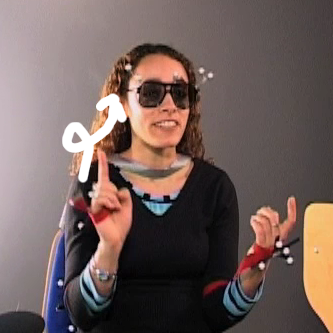
\includegraphics[width=5cm]{figures/treppen-2}
  \caption{\enquote{I think that shall be staircases.}}
  \label{fig:staircases}
\end{figure}

The first syllable of the German noun \textit{Treppen} (\textit{staircases}) carries main stress, indicated by capitalization. 
%
The square brackets indicate the temporal overlap between speech and gesture stroke, which is shown in Figure~\ref{fig:staircases}.
%
The gesture attributes to the noun it attaches to: from the multimodal utterance the observer retrieves the information that the speaker talks about spiral staircases. 
%
This interpretation assumes that the common noun is the affiliate of the iconic gesture.
%
Obviously, mere temporal synchrony is too weak to be an indicator of affiliation.
%
In fact, there are speech-gesture affiliations without temporal overlap between gesture and verbal affiliate at all \citep[e.g.][]{Luecking:Rieser:Stegmann:2004}.
%
Therefore, temporal overlap or vicinity is just one indicator of affiliation, a second one is intonation: a gesture is usually related to a stressed element in speech \citep{McClave:1994,Nobe:2000,Loehr:2004,Loehr:2007}. \is{phonetic speech-gesture constraint}
%
As a result, multimodal communication gives rise to complex \enquote{peak pattern} \citep{Tuite:1993,Loehr:2004,Jannedy:Mendoza-Denton:2005}.


The interpretation of a gesture changes with different affiliations. \is{gesture affiliation}
%
Suppose the gesture from Figure~\ref{fig:staircases} is produced in company to stressed \textit{glaube} (\textit{think}) instead of \textit{staircases}: 
%
\ea \label{ex:think}
\glt Ich G[LAUbe das sollen Trep]pen sein.\\
     I THINK those should stairs be. \\
\glt \enquote{I think those should be stairs.}
\z
%
Now the spiral movement is interpreted as a metaphorical depiction of a psychological process. 
%
Thus, the interpretation of a gesture depends on the integration point (affiliation), which in turn is marked by prosody.
%
Note that the resulting multimodal utterance may express a richer content than speech alone, as in (\ref{ex:staircases}), or a content equivalent to speech content, as in (\ref{ex:think}); it can even express less than speech or contradict speech:\footnote{In case of contradiction, that, speech-gesture mismatch, the resulting multimodal utterance is perceived as ill-formed and induces N400 effects \citep{Wu:Coulson:2005,Kelly:Kravitz:Hopkins:2004}.} \is{gesture-speech relations}
%
\begin{quote}
The nonverbal act can repeat, augment, illustrate, accent, or contradict the words; it can anticipate, coincide with, substitute for or follow the verbal behavior; and it can be unrelated to the verbal behavior.\hfill 
\citep[53]{Ekman:Friesen:1969}
\end{quote}


Given the linguistic significance of gestures as sketched in the preceding sections grammar-oriented accounts on speech-gesture integration have recently been developed that try to deal with (at least one of) the three basic phenomena, though with different settings of priorities, including
%
\citet{Alahverdzhieva:2013}, % diss 
%
\citet{Alahverdzhieva:Lascarides:2010},
%
\cite{Ebert:2014:a},
%
\citet{Giorgolo:2010},
%
\citet{Giorgolo:Asudeh:2011},
%
\citet{Luecking:2013:a}, % diss
%
\citet{Luecking:2016},
%
\citet{Rieser:2008},
%
\citet{Rieser:Poesio:2009},
%
\citet{Rieser:2011},
%
\citet{Rieser:2015},
%
\citet{Schlenker:2018}.
\is{speech-gesture integration|)}

The HPSG-related approaches are briefly reviewed below.
%
For grammars for sign languages see \crossrefchaptert{sign-lg}. \todo{fix crossref}
%
There also belong investigations into iconic features of American Sign Language \citep{Schlenker:Lamberton:Santoro:2013,Schlenker:2014}.




\section{Gestures in HPSG}
\label{sec:gestures-hpsg}


\subsection{Precursors} 
\label{sec:precursors}

Using typed feature structures in order to represent the form and meaning of gestures goes back to computer science approaches to human-computer interaction (HCI). % \citep[cf.][]{Luecking:Pfeiffer:2012}.
%
The \textit{QuickSet} system \citep{Cohen:et:al:1997} allows users to operate on a map and move objects or create barb wires (the project was funded by a grant from the US army) by giving verbal commands and manually indicating coordinates.
%
The system processes voice and pen (gesture) input by assigning signals from both media representations in the form of attribute-value matrices (AVMs) \citep{Johnston:1998,Johnston:et:al:1997}.
%
% The common representation format is a precondition for implementing multimodal integration of speech and gestures in terms of unification \citep[cf.][]{Luecking:Rieser:Staudacher:2006:a}.
%
For instance, \textit{QuickSet} will move a vehicle to a certain location on the map when asked to \textit{Move this[\Pointing] motorbike to here[\Pointing]}, where \enquote*{\Pointing} represents an occurrence of touch gesture (i.e., pen input). 


\is{multimodal chart parser|(}
Since a linguistic unification-based grammar rests on a conventional, \enquote{unimodal} parser, \citet{Johnston:1998} and \citet{Johnston:et:al:1997} developed a \emph{multimodal chart parser}, which are still a topic of computational linguistics \citep{Alahverdzhieva:Flickinger:Lascarides:2012} (see also \textit{Computational linguistics and Language Engineering}, this volume).
%
A multimodal chart parser consists of two or more layers and allows for layer-crossing charts.
%
The multimodal NP \textit{this[\Pointing] motorbike}, for instance, is processed in terms of a multimodal chart parser covering of a speech (s) and a gesture (g) layer:
%
\ea \label{ex:multimodal-chart-parser}
\begin{tikzpicture}[
  baseline, 
  node distance=3cm, 
  shorten >=1pt,
  >=latex,
  State/.style={circle, fill=black, minimum size=6pt, inner sep=0pt}
  ]
  \node (speech) {s:};
  \node [State] (q_0) [right=of speech, label=below:0] {};
  \node [State] (q_1) [right=of q_0, label=below:1]    {};
  \node [State] (q_2) [right=of q_1, label=below:2]    {};
  \path [->] (q_0) edge [bend left]  node [above] {\textsc{det}}  (q_1)
                   edge              node [below] {\textit{this}} (q_1)
                   edge [loop above, min distance=1cm] node {\textsc{np}$\rightarrow$\textsc{.det n}} (q_0)
             (q_1) edge [bend left]  node [above] {\textsc{n}}    (q_2)
                   edge              node [below] {\textit{motorbike}} (q_2);
  \begin{scope}[yshift={-1.5cm}]
    \node (gesture) {g:};
    \node [State] (q_3) [right=5cm of gesture, label=below:3] {};
    \node [State] (q_4) [right=of q_3, label=below:4]     {};
    \path [->] (q_3) edge             node [above] {\Pointing}          (q_4)
                     edge [bend right] node [below] {\textit{pointing}} (q_4);
  \end{scope}
\end{tikzpicture}
\z

A multimodal chart or \emph{multichart} is defined in terms of sets of identifiers from both layers.
%
Possible multicharts from (\ref{ex:multimodal-chart-parser}) include the following ones:
%
\ea
multichart 1: \{[s,0,1], [g,3,4]\} \\
multichart 2: \{[s,1,2], [g,3,4]\} \\
\ldots
\z
\is{multimodal chart parser|)}

% The meaning (\textit{content}) of a gesture of category (\textit{cat}) \textit{spatial\_gesture}  like \enquote*{\Pointing} is represented as a \textit{latitude-longitude} coordinate pair \citep{Johnston:1998}:
% %
% \ea
% \begin{avm}
% \[cat: & \textit{spatial\_gesture} \\
%   content: & \[fsType: & \textit{point} \\
%                coord: & \textit{latlong}$(x,y)$\]
% \]
% \end{avm}
% \z


The basic rule for integrating spatial gestures with speech commands is the \emph{basic integration scheme} \citep{Johnston:1998,Johnston:et:al:1997}, reproduced in (\ref{ex:basic-integration-scheme}): \is{basic integration scheme} \is{multimodal integration scheme}
%
\ea \label{ex:basic-integration-scheme}
\begin{avm}
  \[lhs : & \[cat : & \textit{command} \\
 	modality : & \@2 \\
  	content : & \@1 \\
    time : & \@3\] \\
    rhs : & \[dtr1 : & \[cat : & \textit{located\_command} \\
	modality : & \@6 \\
    content : & \@1[location \@5] \\
    time : & \@7\] \\
    dtr2 : & \[cat : & \textit{spatial\_gesture} \\
    content : & \@5 \\
    modality :& \@9 \\
    time :& \@{10}\]\] \\
    constraints : & \{overlap(\@7,\@{10}) $\lor$ follow(\@7,\@{10},4) \\
    total-time(\@7,\@{10},\@3) \\ 
    assign-modality(\@6,\@9,\@2)\}\]
\end{avm}
\z

The AVM in (\ref{ex:basic-integration-scheme}) implements a mother-daughter structure along the lines of a context free grammar rule, where a left-hand side (\textit{lhs}) expands to a right-hand side (\textit{rhs}).
%
The right-hand  side consists of two constituents (daughters \textit{dtr1} and \textit{dtr2}), a verbal expression (\textit{located\_command}) and a gesture.
%
The semantic integration between both modalities is achieved in terms of feature-structure sharing, see tag \avmbox{5}: 
%
the spatial gesture provides the location coordinate for the verbal command. 

The bimodal integration is constrained by a set of restrictions, mainly regulating the temporal relationship between speech and gesture (see tags \avmbox{7} and \avmbox{10} in the \enquote*{constraints} field): 
%
the gesture may overlap with its affiliated word in time, or follow it in at most four seconds.


An integration scheme akin to that displayed in (\ref{ex:basic-integration-scheme}) also underlies current grammar-oriented approaches to deictic and iconic gestures (see Sections~\ref{sec:pointing-gestures} and \ref{sec:iconic-gestures} below).



\subsection{Representing Gestures with AVMs}
\label{sec:repr-gest-with}

\is{gesture representation|(}
Representing the formal features of gestures in terms of attribute-value matrices has been initiated in robotics \citep{Kopp:Tepper:Cassell:2004}. 
%
A representation format that captures the \enquote{phonological}, physical properties of a gesture is designed according to the moveable junctions of arms and hands.
%
For instance, the representation of the gesture in Figure~\ref{fig:staircases} according to the format used in \citet{Luecking:Bergmann:Hahn:Kopp:Rieser:2010} is given in (\ref{ex:gesture-representation}):

\ea \label{ex:gesture-representation}
\begin{avm}
  \[\asort{right hand}
    HANDSHAPE &\[SHAPE & G \\ 
      PATH & 0 \\
      DIR & 0 \] \\
    PALM & \[ORIENT & PAB>PAB/PUP>PAB\\
      PATH & 0 \\
      DIR & 0 \] \\
    BOH & \[ORIENT & BUP>BTB/BUP>BUP \\
      PATH & ARC>ARC>ARC \\
      DIR & MR>MF>ML\] \\
    WRIST & \[POSITION & P-R\\
      PATH & LINE \\
      DIR & MU \\
      DIST & D-EK\\
      EXTENT & small\]  \\
    SYNC & \[CONFIG & BHA \\
      REL.MOV & LHH \]
  \]
\end{avm}
\z

The formal description of a gestural movement is given in terms of the handshape, the orientations of the palm and the back of the hand (BOH), the movement trajectory (if any) of the wrist and the relation between both hands (synchronicity, SYNC). 
%
The \isi{handshape} is drawn from the \isi{fingerspelling alphabet} of American Sign Language, as illustrated in Figure~\ref{fig:asl}.
%
The orientations of palm and back of hand are specified with reference to the speaker's body (e.g., \textit{PAB} encodes \enquote{palm away from body} and \textit{BUP} encodes \enquote{back of hand upwards}). 
%
Movement features are specified with respect to the wrist: the starting position is given and the performed trajectory is encoded in terms of the described path and the direction and extent of the movement.
%
Position and extent are given with reference to the \emph{gesture space}, that is the structured area within the speaker's immediate reach \citep{McNeill:1992} -- see Figure~\ref{fig:gesture-space}. \is{gesture space}
%
Rectangular and roundish movement are distinguished in terms of \textit{line} or \textit{arc} values of feature DIR(ection).
%
An example is given in Figure~\ref{fig:move-direction}.
%
For a documentation of gesture representation along this line see \citet{FIGURE:annotation}.
%
For related formats see \citet{Martell:Osborn:Friedman:Howard:2002} and \citet{Gibbon:et:al:2003}.
%
For a different approach see \citet{Lausberg:Sloetjes:2009}.


\begin{figure}[tb]
  \centering
  \includegraphics[width=0.5\linewidth]{figures/ASL_alphabet_gallaudet}
  \caption[ASL]{American Sign Language fingerspelling alphabet (image released to Public Domain by user Ds13 in the English Wikipedia at \printdate{2018-12-18}).}
  \label{fig:asl}
\end{figure}

\begin{figure}[tb]
  \centering
  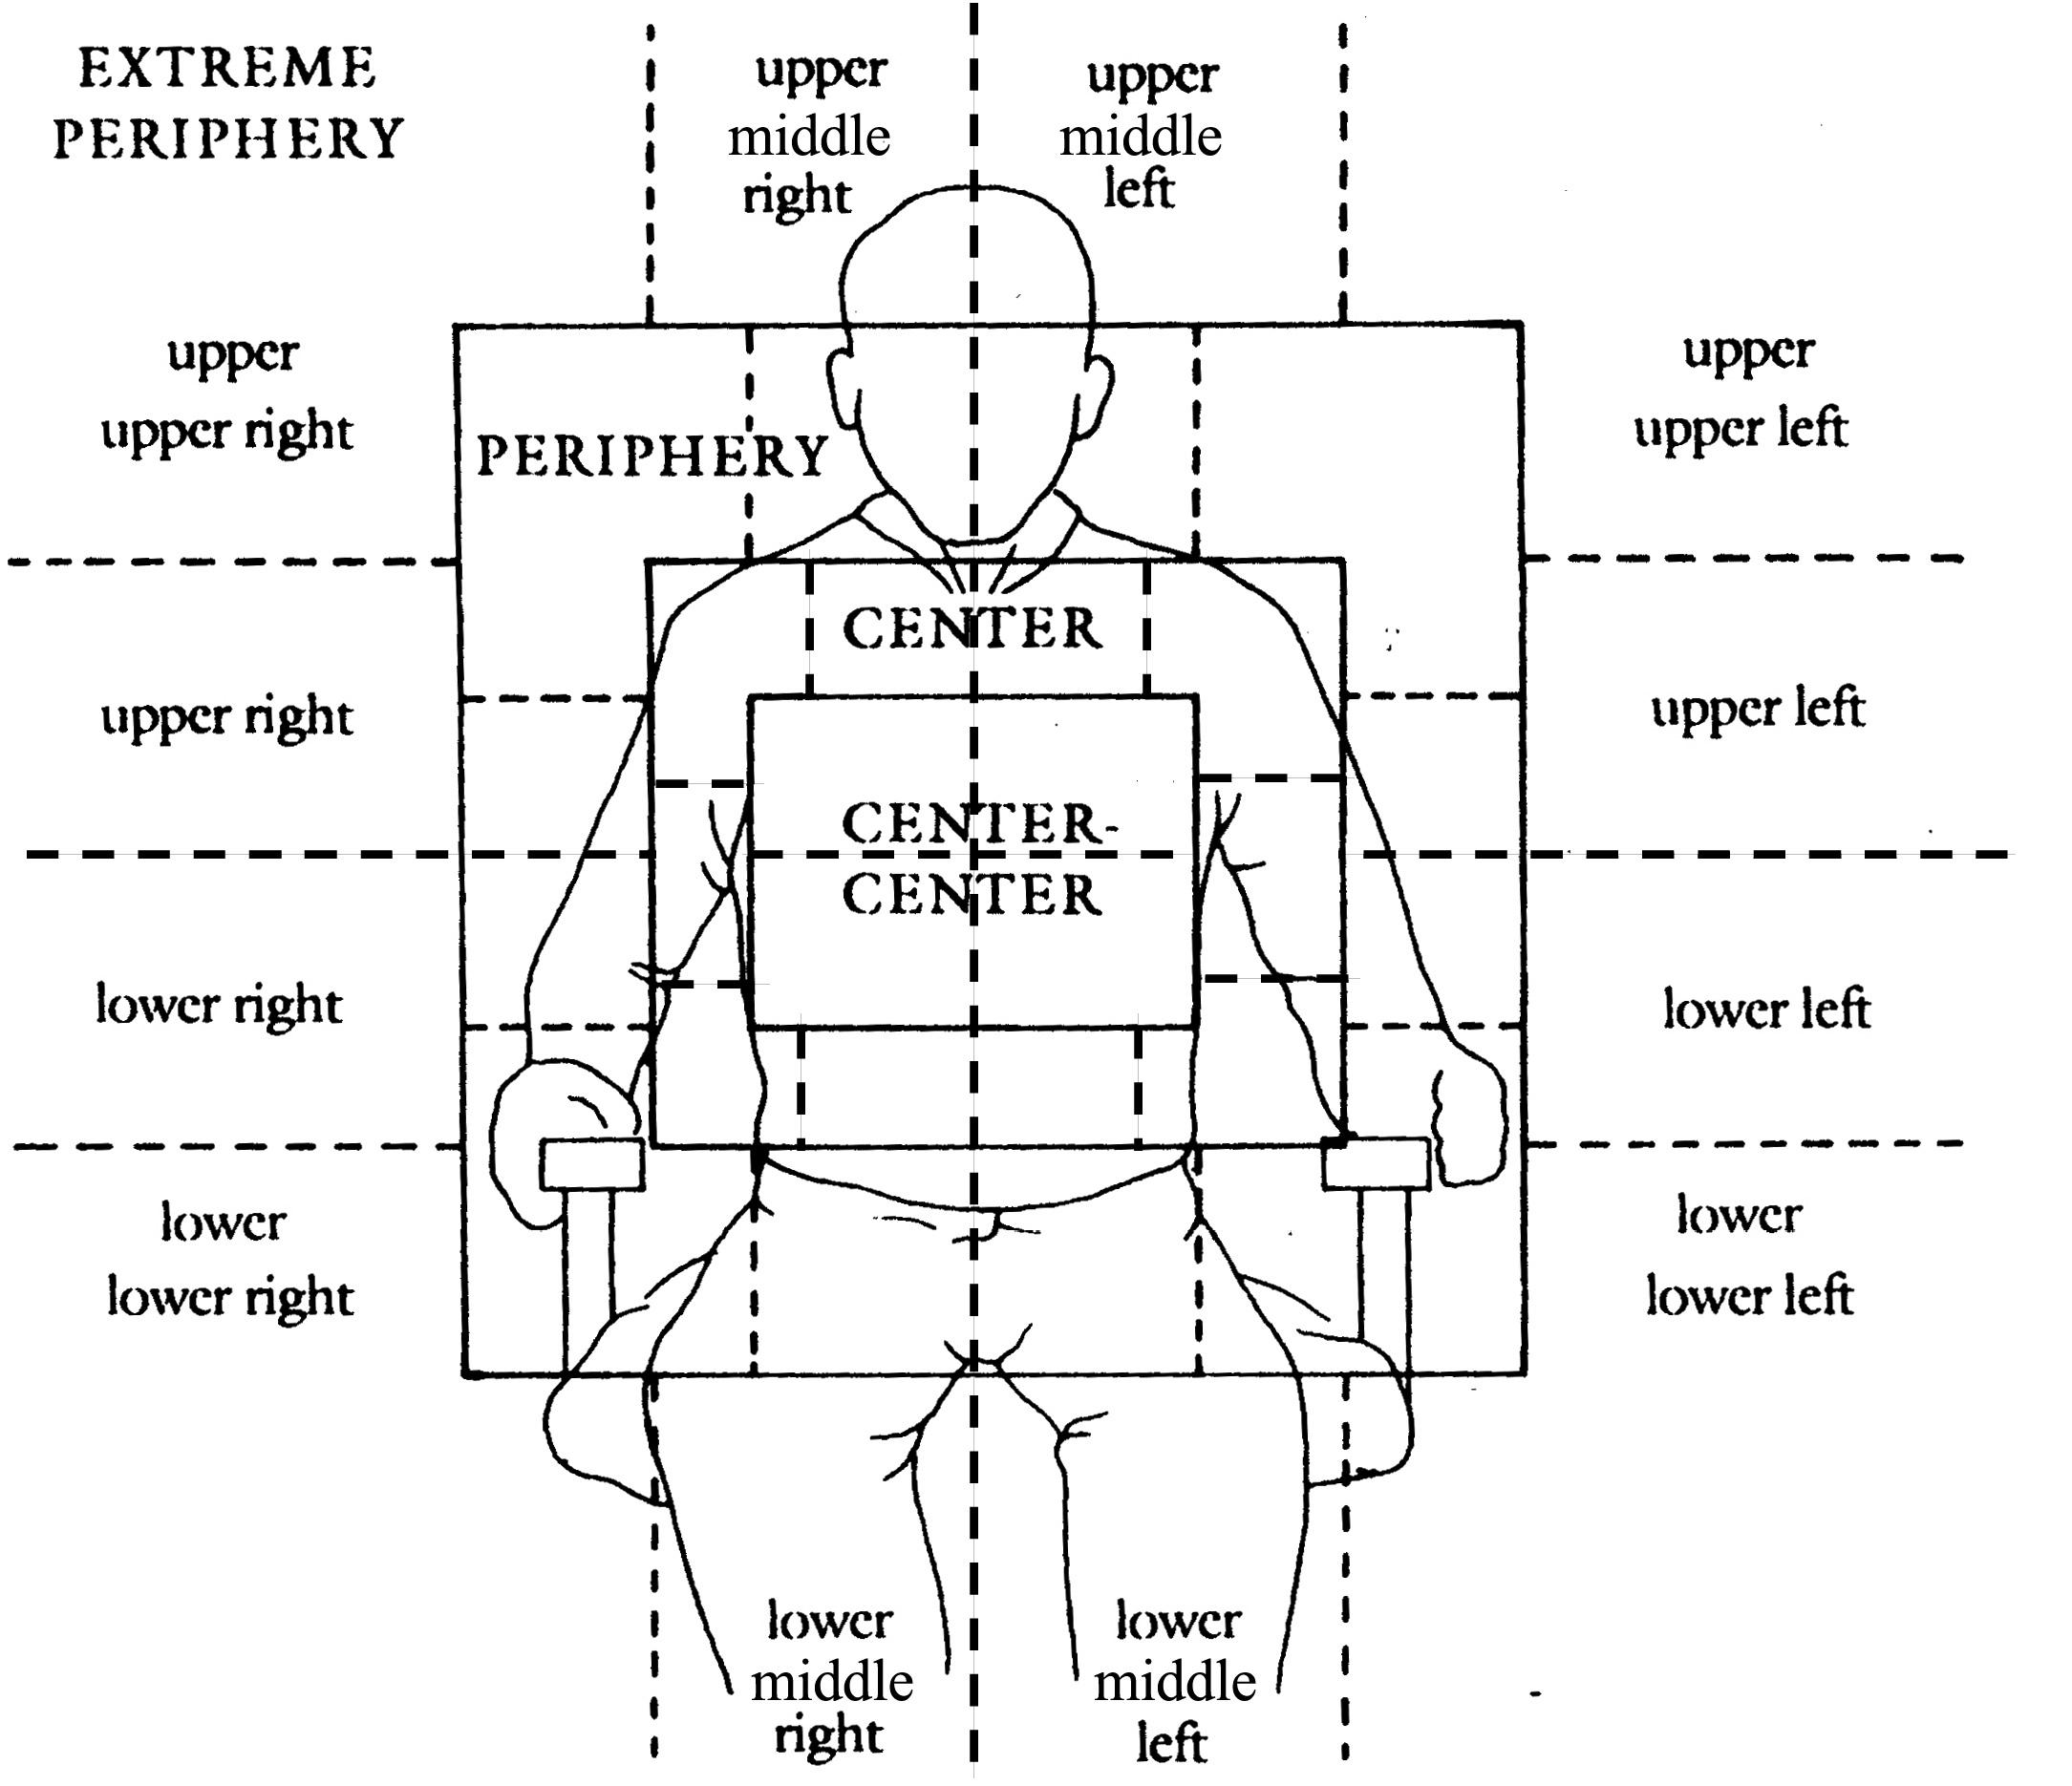
\includegraphics[width=0.5\linewidth]{figures/gesture-space}
  \caption[Gesture Space]{Gesture Space (taken from \citet[378]{McNeill:1992}.)}
  \label{fig:gesture-space}
\end{figure}


\begin{figure}[tb]
  \centering
  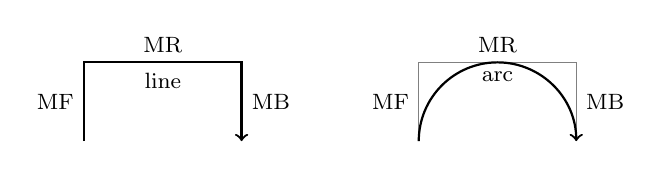
\begin{tikzpicture}[baseline, move/.style={font=\footnotesize, midway, text=black}]
    \draw [thick, ->] (0,-1) -- node [move, left] {MF} (0,0) -- node [move, above] {MR} node [move, below] {line} (2,0) -- node [move, right] {MB} (2,-1);
    \begin{scope}[xshift=4.25cm]
      \draw [thin, gray] (0,-1) -- node [move, left] {MF} (0,0) -- node [move, above] {MR} node [move, below] {arc} (2,0) -- node [move, right] {MB} (2,-1);
      \draw [thick, ->] (0,-1) arc[start angle=180, end angle=0, radius=1];
    \end{scope}
  \end{tikzpicture}
  \caption{The same sequence of direction labels can give rise to an open rectangle or a semicircle, depending on the type of concatenation (example taken from \citet{Luecking:2016}).}
  \label{fig:move-direction}
\end{figure}


The \enquote{phonological} representation of gestures is slightly refined in \citet{Luecking:2016}, where gestures are analysed in terms of a formal event framework \citep{Fernando:2011,Cooper:Ginzburg:2015} in order to account for Gestalt properties of gesture movements (see also the example discussed by \citet{Rieser:2008}).
\is{gesture representation|)}



\subsection{Pointing Gestures}
\label{sec:pointing-gestures}

\is{pointing gesture|(} \is{deictic gesture|(}
Pointing gestures are \emph{the} referring device:
%
they probably pave a way to reference in both an evolutionary and language acquisition perspective. \citep{Bruner:1998,Masataka:2003,Matthews:Behne:Lieven:Tomasello:2012};
%
they are predominant inhabitants of the \enquote{deictic level} of language, interleaving the symbolic (and the iconic) ones (\citet{Levinson:2008}, see also \citet{Buehler:1934:ORIG});
%
they underlie reference in \textit{Naming Games} in computer simulation approaches \citep{Steels:1995} (for a semantic assessment of naming and categorisation games see \citet{Luecking:Mehler:2012}). \is{naming game} \is{categorisation game}
%
The referential import of pointing gesture has been studied experimentally to some detail \citep{Bangerter:Oppenheimer:2006,Kranstedt:Luecking:Pfeiffer:Rieser:Wachsmuth:2006:a,van:der:Sluis:Krahmer:2007}. 
%
As a result, it turns out that pointings do not rest on a direct \enquote{laser}- or \enquote{beam} mechanism \citep{McGinn:1981}.
%
Rather, they serve a (more or less rough) locating function \citep{Clark:1996} that can be modelled in terms of a \emph{pointing cone} \citep{Luecking:Pfeiffer:Rieser:2015}. \is{pointing cone}
%
These works provide an answer to the first basic question (cf. Section~\ref{sec:empir-desid-gramm}): pointing gestures have a \enquote{spatial meaning} which focuses or highlights a region in relation to the direction of the pointing device.
%
Such a spatial semantic model has been introduced in \citet{Rieser:2004} under the name of \emph{region pointing}, where the gesture adds a locational constraint to the restrictor of a noun phrase.
%
The spatial model is also adopted in \citet{Lascarides:Stone:2009:a}, where the region denoted by a pointing is represented by a vector $\vec{p}$.
%
This region is an argument to function $\nu$, however, which maps the projected cone region to $\nu(\vec{p})$, the space-time talked about, which may be different from the gesture space (many more puzzles of local deixis are collected by \citet{Klein:1978} and \citet{Fricke:2007:a}).


Let us illustrate some aspects of pointing gesture integration by means of a real world example (taken from dialogue V5 of the SaGA corpus \citep{Luecking:Bergmann:Hahn:Kopp:Rieser:2010}).
%
The speaker in (\ref{ex:drivetowards}) and Figure~\ref{fig:drivetowards} places a pond with his left hand into gesture space.
%
He then points at his left hand/the pond (on \emph{dual points} see \citet{Goodwin:2003}, on \emph{deferred reference} see \citet{Quine:1950,Nunberg:1993}), depicting \textit{driving towards} or \textit{heading straight}.
%
The movement aspect is subsequently enacted by moving the right hand/driver towards the left hand/pond.
%
\ea \label{ex:drivetowards}
\glt wenn du dort eingefahren bist, fährst Du geradeaus auf einen Teich zu .. 'n Teich .. und .. [\textit{gesture from Figure~\ref{fig:drivetowards} occurs here}] 
\glt \textit{when you drive in there , you're heading straight for a pond .. a pond .. and .. } [\textit{gesture from Figure~\ref{fig:drivetowards} occurs here}] 
\z 

\begin{figure}[tb]
  \centering
  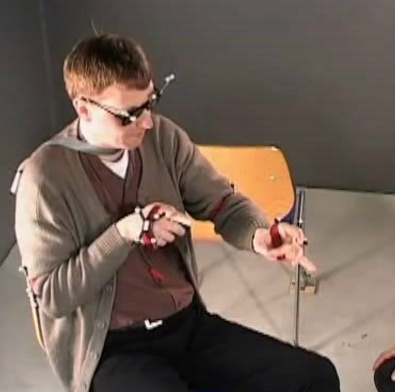
\includegraphics[width=0.5\linewidth]{figures/draufzu}
  \caption{Driving towards/heading straight}
  \label{fig:drivetowards}
\end{figure}

This example highlights two crucial phenomena: firstly, the region pointed at is not the region referred to. 
%
The indicated location in gesture space has to be mapped onto a spatial area of the described situation.
%
Such mapping are accounted for by $\nu(\vec{p})$.
%
Secondly, the gesture is produced \emph{after} speech. 
%
This means that in order to identify the gesture's verbal attachment site something beyond mere temporal synchrony (the second basic question, see Section~\ref{sec:empir-desid-gramm}) has to be exploited.
%
To this end, phonological information on top  of the basic integration scheme in (\ref{ex:basic-integration-scheme}) are used \citep{Alahverdzhieva:Lascarides:2011,Luecking:2013:a}.
%
Within a temporal window (basic integration scheme), a pointing gesture is affiliated to a stressed expression. \is{phonetic speech-gesture constraint}
%
This relaxation captures also post-speech gestures \is{post-speech gesture} as in example (\ref{ex:drivetowards})/Figure~\ref{fig:drivetowards}.
%
Within HPSG, such constraints can be formulated within an interface to metrical trees from the phonological model of \citet{Klein:2000} or phonetic information packing from \citet{Engdahl:Vallduvi:1996} -- \crossrefchaptert{phonology}. \todo{fix crossref}
%
In order to deal with gestures that are affiliated with expressions that are larger than single words, \citet{Alahverdzhieva:Lascarides:2011} also develop a phrase or sentence level integration scheme, where the stressed element has to be a semantic head (in the study of \citet{Mehler:Luecking:2012:d} 18.8\% of the gestures had a phrasal affiliate).
%
On this account, semantic integration of gesture location and verbal meaning (the third basic question from Section~\ref{sec:empir-desid-gramm}) is brought about using underspecification mechanism of \textit{Multiple Recursion Semantics} (MRS) \citep{Copestake:Flickinger:Pollard:Sag:2005}.


(Pointing) gestures that occur in company to a demonstrative expression in speech have received special attention, since they manifest the transition point between the symbolic realm of language and the deictic realm of perception \citep{Levinson:2008,Fricke:2012}.
%
Building on this phenomenon, \citet{Ebert:2014:a,Ebert:Ebert:2016} argue within in a dynamic semantic framework that co-demonstrative gestures \is{co-demonstrative gesture} contribute to at-issue content while other gestures % (called \enquote{contingent} in \citet{Luecking:2013:a} and \enquote{background} in \citet{Cooperrider:2017}) 
contribute to non-at-issue content.
%
Within a presuppositional framework, this picture has been refined due to gestures that are entailed in local contexts in terms of \enquote{cosuppositions} \citet{Schlenker:2018}.


A dialogue-oriented focus is taken in \citet{Luecking:2018:a}: here pointing gesture play a role in formulating processing instructions that guide the addressee in understanding demonstrative noun phrases (see also \crossrefchaptert{pragmatics}).  \todo{fix crossref}


Semantic aspects of iconic features of pointing as discourse referent indication in American Sign Language have been investigated and formally modelled by \citet{Schlenker:Lamberton:Santoro:2013,Schlenker:2014}.
\is{pointing gesture|)} \is{deictic gesture|)}



\subsection{Iconic Gestures}
\label{sec:iconic-gestures}

\is{iconic gesture|(} \is{representational gesture|(}
There is nearly no semantic work on how and which meanings can be assigned to iconic gestures (first basic question from Section~\ref{sec:empir-desid-gramm}).
%
Two exceptions being the approaches of \citet{Rieser:2010} and \citet{Luecking:2013:a,Luecking:2016}.
%
\citet{Rieser:2010} tries to extract a \enquote{depiction typology} out of a speech-and-gesture corpus where formal gesture features are correlated with topological clusters consisting of geometrical constructs. \is{gesture typology}
%
These geometrical objects are used in order to provide a possibly underspecified semantic representation for iconic gestures which is integrated into word meaning \citep{Hahn:Rieser:2010,Rieser:2011}.
%
\citet{Luecking:2013:a,Luecking:2016} draws on Goodman's notion of \emph{exemplification} \citep{Goodman:1976}, iconic gestures are connected to semantic predicates in terms of a reversed denotation relation: the meaning of an iconic gesture is given in terms of the set of predicates which have the gesture event within their denotation. \is{exemplification}
%
In a further step, common perceptual features are extracted and represented as part of a lexical extension of lexemes. 
%
This conception is motivated by psychophysic theories of the perception of biological events \citep{Johansson:1973}, draws on philosophical \isi{similarity} conception beyond isomorphic mappings \citep{Peacocke:1987},\footnote{That mere resemblance, usually associated with iconic signs, is too empty a notion to provide the basis for a signifying relation has been emphasised on various occasions \citep{Burks:1949,Bierman:1962,Eco:1976,Goodman:1976,Sonesson:1998}.} and, using a somewhat related approach at least, has been proven to work in robotics \citep{Sowa:2006:a}.
%
These perceptual features serve as the integration locus for iconic gestures, using standard unification techniques. 
%
With regard to conventionalized sign language, iconic aspects have also been captured in terms of presuppositions that map, for instance, height specifications of signed loci to social properties and relations like power (that is, a higher locus indicates more power) \citep{Schlenker:Lamberton:Santoro:2013}.


The richer formal, functional and representational features of iconic gestures as compared to deictic gestures (cf. Section~\ref{sec:pointing-gestures}) is accounted for in \citet{Alahverdzhieva:Lascarides:2010} by assigning a formal predicate to each \enquote{phonological} feature of a gesture representation (cf. Section~\ref{sec:repr-gest-with}). 
%
These formal gesture predicates are highly underspecified, using \textit{Robust Multiple Recursion Semantics} (RMRS) \citep{Copestake:2007}.
%
That is, they can be assigned various (so far postulated) predicates (which are assumed to be constrained by iconicity \citep{Alahverdzhieva:Lascarides:2010}) with differing arity in the gesture resolution process.
%
Similar to pointing gesture integration, phonetic constraints on word and sentence level apply and semantic integration is achieved using underspecification techniques of \textit{Multiple Recursion Semantics} (MRS) \citep{Copestake:Flickinger:Pollard:Sag:2005}.
%
The received integrated representation are then resolved using the SDRT tools of \citet{Lascarides:Stone:2009:a}.



Iconic gestures in particular are involved in a short-term dynamic phenomenon:
%
on repeated co-occurrence, iconic gestures and affiliated speech can fuse into a \emph{multimodal ensemble} \citep{Kendon:2004,Luecking:Mehler:Menke:2008,Mehler:Luecking:2012:d}. \is{multimodal ensemble} \is{speech-gesture ensemble}
%
The characteristic feature of such an ensemble is that their gestural part, their verbal part, or even both parts can be simplified without changing the meaning of the ensemble.
%
Ensembles, thus, are the result of a process sign formation as studied, for instance, in experimental semiotics \citet{Galantucci:Garrod:2011}.
%
Such grammaticalisation process eventually might lead to conventional signs.
%
However, most conventional, emblematic everyday gesture seem to be the result of circumventing a taboo: something you should not name is gesticulated \citep{Posner:2002}.
\is{iconic gesture|)} \is{representational gesture|)}



\section{Outlook}
\label{sec:outlook}

What are (still) challenging issues with respect to grammar-gesture integration, in particular from a semantic point of view? Candidates include:

\begin{itemize}
\item gestalt phenomena: the trajectories described by a gesture are often incomplete and have to be completed by drawing on gestalt principles or everyday knowledge \citep{Luecking:2016};
\item negligible features: not all formal features of a gesture are meaning"=carrying features in the context of utterance. For instance, in a dynamic gesture the handshape often (though not always) does not provide any semantic information. How to distinguish between significant and negligible gesture features?
\item \enquote{semantic endurance}: due to holds, gestural meanings can kept fixed for some time is keeps available for semantic attachment. This may call for a more sophisticated algebraic treatment of speech-gesture integration than offered by typed feature structures \citep{Rieser:2015}.
\end{itemize}

Finally, the empirical domain of \enquote{gesture} has to extended to other non-verbal signals such as laughter \citep{Ginzburg:Breitholz:Cooper:Hough:Tian:2015}, facial expressions or gaze (see Section~\ref{sec:why-gestures} for a brief list of non-verbal signals), in isolation as well as in mutual combination.
%
Thus, there is still some way to go in order to achieve a fuller understanding of natural language interaction and thereby natural languages.


 
% \section*{Abbreviations}
% \section*{Acknowledgements}

\avmoptions{active}

{\sloppy
\printbibliography[heading=subbibliography,notkeyword=this]
}
\end{document}
